% This is the Duke University Statistical Science LaTeX thesis template.
% It has been adapted from the Reed College LaTeX thesis template. The
% adaptation was done by Mine Cetinkaya-Rundel (MCR). Some of the comments
% that are specific to Reed College have been removed.
%
% Most of the work on the original Reed College document class and template
% was done by Sam Noble (SN). Later comments etc. by Ben Salzberg (BTS).
% Additional restructuring and APA support by Jess Youngberg (JY).
%
% See https://www.reed.edu/cis/help/latex/ for help. There are a
% great bunch of help pages there, with notes on
% getting started, bibtex, etc. Go there and read it if you're not
% already familiar with LaTeX.
%
% Any line that starts with a percent symbol is a comment.
% They won't show up in the document, and are useful for notes
% to yourself and explaining commands.
% Commenting also removes a line from the document;
% very handy for troubleshooting problems. -BTS

%%
%% Preamble
%%
% \documentclass{<something>} must begin each LaTeX document
\documentclass[12pt,twoside]{dukestatscithesis}
% Packages are extensions to the basic LaTeX functions. Whatever you
% want to typeset, there is probably a package out there for it.
% Chemistry (chemtex), screenplays, you name it.
% Check out CTAN to see: http://www.ctan.org/
%%
\usepackage{graphicx,latexsym}
\usepackage{amsmath}
\usepackage{amssymb,amsthm}
\usepackage{longtable,booktabs,setspace}
\usepackage{chemarr} %% Useful for one reaction arrow, useless if you're not a chem major
\usepackage[hyphens]{url}
% Added by CII
\usepackage{hyperref}
\usepackage{lmodern}
\usepackage{float}
\floatplacement{figure}{H}
% End of CII addition
\usepackage{rotating}

% Next line commented out by CII
%%% \usepackage{natbib}
% Comment out the natbib line above and uncomment the following two lines to use the new
% biblatex-chicago style, for Chicago A. Also make some changes at the end where the
% bibliography is included.
%\usepackage{biblatex-chicago}
%\bibliography{thesis}


% Added by CII (Thanks, Hadley!)
% Use ref for internal links
\renewcommand{\hyperref}[2][???]{\autoref{#1}}
\def\chapterautorefname{Chapter}
\def\sectionautorefname{Section}
\def\subsectionautorefname{Subsection}
% End of CII addition

% Added by CII
\usepackage{caption}
\captionsetup{width=5in}
% End of CII addition

% \usepackage{times} % other fonts are available like times, bookman, charter, palatino


% To pass between YAML and LaTeX the dollar signs are added by CII
\title{Matrix Completion Techniques For Anomaly Detection in Network Attacks}
\author{James C. Wu}
% The month and year that you submit your FINAL draft TO THE LIBRARY (May or December)
\date{May 2018}
\advisor{Peter D. Hoff}
\institution{Duke University}
\degree{Bachelor of Science in Statistical Science}
\committeememberone{Jerry P. Reiter}
\committeemembertwo{Galen Reeves}
\dus{Mine Cetinkaya-Rundel}
%If you have two advisors for some reason, you can use the following
% Uncommented out by CII
% End of CII addition

%%% Remember to use the correct department!
\department{Department of Statistical Science}

% Added by CII
%%% Copied from knitr
%% maxwidth is the original width if it's less than linewidth
%% otherwise use linewidth (to make sure the graphics do not exceed the margin)
\makeatletter
\def\maxwidth{ %
  \ifdim\Gin@nat@width>\linewidth
    \linewidth
  \else
    \Gin@nat@width
  \fi
}
\makeatother

\renewcommand{\contentsname}{Table of Contents}
% End of CII addition

\setlength{\parskip}{0pt}

% Added by CII
  %\setlength{\parskip}{\baselineskip}
  \usepackage[parfill]{parskip}

\providecommand{\tightlist}{%
  \setlength{\itemsep}{0pt}\setlength{\parskip}{0pt}}

\Acknowledgements{
I thank my advisor, Professor Peter Hoff, and the Director of
Undergraduate Studies, Professor Mine Cetinkaya-Rundel, for their
guidance in this project. I also thank Duke University's Statistics
Department for supervising this project and the Office of Information
Technology for providing the dataset. Most of all I thank my parents for
their continued unwavering support in all my endeavors.
}

\Dedication{

}

\Preface{

}

\Abstract{
The goal of this paper is to identify novel methods for detecting
anomalies in network IP data. The data is comprised of four continuous
features (source bytes, destination bytes, source packets, destination
packets) divided by their respective source port and destination port
combinations. Thus, the data is represented as a 3-dimensional tensor
\(T \in \mathbb{R}^{m \times n \times 4}\), where \(m\) is the number of
source ports, \(n\) is the number of destination ports, and \(4\) is the
number of continuous features. Each cell in \(T\), \(t_{ijk}\) stores
the mean of the observations of continuous feature \(k\) between source
port at index \(i\) and destination port at index \(j\). This paper
proposes three techniques for generating means to fill in the missing
cells in \(T\), thereby completing the tensor, so as to provide
reasonable estimates for new observations between every possible port
combination. In the context of anomaly detection, new observations
between ports that do not align closely with their corresponding
estimate in \(T\) are considered anomalies. The first technique uses a
low-rank singular value decomposition algorithm for completing
individual matrix slices of the tensor. The second defines a statistical
model for the values in \(T\) and uses a Bayesian Gibbs Sampling
Procedure to simulate missing values in individual matrix slices of
\(T\). Finally, the third approach extends the first and second
approaches to completing the tensor all at once, rather than with
completing individual matrices.
}

% End of CII addition
%%
%% End Preamble
%%
%

\usepackage{amsthm}
\newtheorem{theorem}{Theorem}[chapter]
\newtheorem{lemma}{Lemma}[chapter]
\theoremstyle{definition}
\newtheorem{definition}{Definition}[chapter]
\newtheorem{corollary}{Corollary}[chapter]
\newtheorem{proposition}{Proposition}[chapter]
\theoremstyle{definition}
\newtheorem{example}{Example}[chapter]
\theoremstyle{definition}
\newtheorem{exercise}{Exercise}[chapter]
\theoremstyle{remark}
\newtheorem*{remark}{Remark}
\newtheorem*{solution}{Solution}
\begin{document}

% Everything below added by CII
  \maketitle

\frontmatter % this stuff will be roman-numbered
\pagestyle{empty} % this removes page numbers from the frontmatter
  \begin{acknowledgements}
    I thank my advisor, Professor Peter Hoff, and the Director of
    Undergraduate Studies, Professor Mine Cetinkaya-Rundel, for their
    guidance in this project. I also thank Duke University's Statistics
    Department for supervising this project and the Office of Information
    Technology for providing the dataset. Most of all I thank my parents for
    their continued unwavering support in all my endeavors.
  \end{acknowledgements}

  \hypersetup{linkcolor=black}
  \setcounter{tocdepth}{2}
  \tableofcontents


  \begin{abstract}
    The goal of this paper is to identify novel methods for detecting
    anomalies in network IP data. The data is comprised of four continuous
    features (source bytes, destination bytes, source packets, destination
    packets) divided by their respective source port and destination port
    combinations. Thus, the data is represented as a 3-dimensional tensor
    \(T \in \mathbb{R}^{m \times n \times 4}\), where \(m\) is the number of
    source ports, \(n\) is the number of destination ports, and \(4\) is the
    number of continuous features. Each cell in \(T\), \(t_{ijk}\) stores
    the mean of the observations of continuous feature \(k\) between source
    port at index \(i\) and destination port at index \(j\). This paper
    proposes three techniques for generating means to fill in the missing
    cells in \(T\), thereby completing the tensor, so as to provide
    reasonable estimates for new observations between every possible port
    combination. In the context of anomaly detection, new observations
    between ports that do not align closely with their corresponding
    estimate in \(T\) are considered anomalies. The first technique uses a
    low-rank singular value decomposition algorithm for completing
    individual matrix slices of the tensor. The second defines a statistical
    model for the values in \(T\) and uses a Bayesian Gibbs Sampling
    Procedure to simulate missing values in individual matrix slices of
    \(T\). Finally, the third approach extends the first and second
    approaches to completing the tensor all at once, rather than with
    completing individual matrices.
  \end{abstract}

\mainmatter % here the regular arabic numbering starts
\pagestyle{fancyplain} % turns page numbering back on

The goal of this paper is to identify novel methods for detecting
anomalies in network IP data. The data is comprised of four continuous
features (source bytes, destination bytes, source packets, destination
packets) divided by their respective source port and destination port
combinations. Thus, the data is represented as a 3-dimensional tensor
\(T \in \mathbb{R}^{m \times n \times 4}\), where \(m\) is the number of
source ports, \(n\) is the number of destination ports, and \(4\) is the
number of continuous features. Each cell in \(T\), \(t_{ijk}\) stores
the mean of the observations of continuous feature \(k\) between source
port at index \(i\) and destination port at index \(j\). This paper
proposes three techniques for generating means to fill in the missing
cells in \(T\), thereby completing the tensor, so as to provide
reasonable estimates for new observations between every possible port
combination. In the context of anomaly detection, new observations
between ports that do not align closely with their corresponding
estimate in \(T\) are considered anomalies. The first technique uses a
low-rank singular value decomposition algorithm for completing
individual matrix slices of the tensor. The second defines a statistical
model for the values in \(T\) and uses a Bayesian Gibbs Sampling
Procedure to simulate missing values in individual matrix slices of
\(T\). Finally, the third approach extends the first and second
approaches to completing the tensor all at once, rather than with
completing individual matrices.

\chapter{Introduction}\label{introduction}

\section{Anomaly Detection}\label{anomaly-detection}

Anomaly detection is used to identify unusual patterns or observations
that do not conform to expected behavior in a dataset. Anomalies can be
broadly categorized into three categories:

Point anomalies: A single instance of data is anomalous if it's too far
off from the rest. For example detecting credit card fraud based on a
single spending spree that represents the credit card being stolen and
used.

Contextual anomalies: The abnormality is context specific. This type of
anomaly is common in time-series data. For instance, high spending on
food and gifts every day during the holiday season is normal, but may be
considered unusual otherwise.

Collective anomalies: A set of data observations that when collectively
assessed helps in detecting anomalies. For instance, repeated pings from
a certain IP address to a port connection on a hosted network may be
classified as a port scanner, which often preludes a network attack.

\section{Network Attacks}\label{network-attacks}

Network security is becoming increasingly relevant as the flow of data,
bandwith of transactions, and user dependency on hosted networks
increase. As entire networks grow in nodes and complexity, attackers
gain easier entry points of access to the network. The most benign of
attackers attempt to shutdown networks (e.g.~causing a website to
shutdown with repeated pings to its server), while more malicious
attempts involve hijacking the server to publish the attacker's own
content or stealing unsecured data from the server, thus compromising
the privacy of the network's users.

Attackers follow a specific three step strategy when gathering
intelligence on a network, the most important component of which is
scanning. Network scanning is a procedure for identifying active hosts
on a network, the attacker uses it to find information about the
specific IP addresses that can be accessed over the Internet, their
target's operating systems, system architecture, and the services
running on each node/computer in the network. Scanning procedures, such
as ping sweeps and port scans, return information about which IP
addresses map to live hosts that are active on the Internet and what
services they offer. Another scanning method, inverse mapping, returns
information about what IP addresses do not map to live hosts; this
enables an attacker to make assumptions about viable addresses.

All three of these scanning methods leave digital signatures in the
networks they evaluate because they apply specific pings that are then
stored in the network logs. Most scanners use a specific combination of
bytes, packets, flags (in TCP protocol), and ports in a sequence of
pings to a network. Identifying a scanner's often many IP addresses from
the set of pings available in the network's logs is thus an anomaly
detection problem. In particular, because the data is unlabeled, meaning
it is unclear which observations are actually scanners and which are
just standard user behavior, unsupervised approaches are necessary for
tackling the problem.

\section{Network Dataset}\label{network-dataset}

This particular dataset is from Duke University's Office of Information
Technology (OIT), and it covers all observations in their network
traffic during a five minute period in February 2017.

\subsection{Features}\label{features}

The networks dataset contains 13 features, 8 categorical and 5
continuous, and the observations are unlabeled (not specified whether
they are considered a scanner). The 13 features are:

\textbf{Continuous:}
\begin{itemize}
\tightlist
\item
  StartTime (Start Time): the time when the observation is logged
\item
  SrcBytes (Source Bytes): the total number of bytes sent in the
  observation
\item
  SrcPkts (Source Packets): the number of packets sent in the
  observation
\item
  DstBytes (Destination Bytes): the total number of bytes received in
  the observation
\item
  DstPkts (Destination Packets): the number of packets received in the
  observation Note, the destination packets and bytes features do not
  have the same values as their source counterparts because the
  connections are compressed and decompressed into different forms and
  byte sizes when sent. For instance, it is possible for the number of
  destination packets to be larger than source packets. It is also
  possible for information to be lost during the connection.
\end{itemize}
\textbf{Categorical:}
\begin{itemize}
\tightlist
\item
  Flgs (connection flag): flow state flags seen in transaction between
  the two addresses
\item
  Proto (network protocol): specifies the rules used for information
  exchange via network addresses. Transmission Control Protocol (TCP)
  uses a set of rules to exchange messages with other Internet points at
  the information packet level, and Internet Protocol (IP) uses a set of
  rules to send and receive messages at the Internet address level.
\item
  SrcAddr (Source Address): the IP address of the connection's source
\item
  DstAddr (Destination Address): the IP address of the connection's
  destination
\item
  Sport (Source Port): the network port number of the connection's
  source. A port numbers identifies the specific process to which a
  network message is forwarded when it arrives at a server.
\item
  Dport (Destination Port): the network port number of the connection's
  destination
\item
  Dir (direction): the direction of the connection
\item
  State (connection state): a categorical assessment of the current
  phase in the transaction when the timestamp is recorded
\end{itemize}
Note, the addresses have been anonymized for security reasons.

\subsection{Argus}\label{argus}

Argus is the open source network security tool applied to network
transactions that collects the data for the features. The Argus wiki and
the OIT manual provides key insights into the structure and nature of
the data. Specifically, the sessions are clustered together by address,
so the pytes and packets values are accumulative over a set duration and
each session has its own start time but does not have a tracked end
time. There exist 2-4 million connections on average every 5 minutes.
Furthermore the protocol in this dataset is always gathered from TCP
protocol and the direction will always be to the right (i.e.~Source to
Destination). This information supports dropping proto, StartTime, and
Direction from the dataset for future analysis because they do not
present any information regarding whether an observation can be
considered an anomaly. Furthermore, the State feature may not be
reliable because Argus occasionally resets the state data statistics
during monitoring.

\subsection{Status Quo Solution}\label{status-quo-solution}

OIT's current solution for detecting scanners relies on specific domain
knowledge gathered from diagnostics programs and data analysis completed
on previous data. They prevent scanners by blocking IP addresses that
fit certain rules they have constructed to run on every network
transaction as it occurs. The specific checks in these rules are private
for security reasons, but they belong to the nature of evaluating the
size of transactions, repeated connections between particular ports,
many pings from the same address, and combinations of these particular
behaviors.

While this solution presents a methodical way for banning IP addresses
and its method of rule checking is essentially removing what OIT
considers outliers for network transactions-any observation that does
not fit within the constraints specified by the rules is classified as
an outlier and its source IP is blocked-it is inflexible, prone to
detecting false negatives, and fails to detect observations that may be
within the parameter constraints of the rules but are anomalous with
respect to other parameters or parameter constraints.

\section{Problem Formulation}\label{problem-formulation}

Preliminary data analysis signaled that there may exist trends between
different port combinations. For instance, a particular source and
destination port may frequently contain large byte transactions in their
connections. Devising a systematic way to identify these combinations
may present outliers that can be further investigated for scanner
behavior.

This approach to the anomaly detection problem reduces the dataset to
the values of the four continuous features, SrcBytes, SrcPkts, DstBytes,
DstPkts, observed across different source port and destination port
combinations. The data can be represented as a 3-dimensional tensor
\(T \in \mathbb{R}^{m \times n \times 4}\) where \(m\) represents the
number of source ports, \(n\) represents the number of destination
ports, and \(4\) accounts for the four continuous features in the
dataset. Each cell, \(t_{ijk}\), contains the mean of all the
observations observed between the source port at index \(i\) and
destination port at index \(j\). In the cases where the combination of
\(i\) and \(j\) is not observed in the dataset, \(t_{ijk}\) is
considered missing (NA). Note, the data is collected in a way where
either all four continuous features are observed, or none are observed,
i.e.~a missing cell, \(t_{ij1}\) indicates
\(t_{ij2}, t_{ij3} and t_{ij4}\) are also missing.

The goal of this paper is to devise and assess strategies for
calculating a reasonable estimate for the missing cells in \(T\) to
create the completed tensor \(T' \in \mathbb{R}^{m \times n \times 4}\).
As new observations are observed for combinations of source ports at
index \(i\) and destination ports at index \(j\), the \(t'_{ijk}\)
values can be interpreted as an approximation for the expected behavior
for that particular port combination. Observations with continuous
features that are a certain threshold away from \(t'_{ijk}\) may be
marked as anomalies and investigated further.

\section{Introduction of Methods}\label{introduction-of-methods}

Chapters 3,4, and 5 discuss three methods for completing the tensor
\(T\). The first two techniques slice \(T\) into four matrices divided
by the four continuous features:
\(Y^{(1)}, Y^{(2)}, Y^{(3)}, Y^{(4)} \in \mathbb{R}^{m \times n}\).
Because both techniques apply to each matrix separately, the techniques
will refer to a general matrix \(Y\), which represents any of
\(Y^{(1)}, Y^{(2)}, Y^{(3)}, Y^{(4)}\). Each \(Y^{(k)}\) has missingness
because not every source port interacts with every destination port.
Chapter three considers an iterative approach using an alternating least
squares technique and the best low-rank approximation of \(Y\) to
repeatedly calculate estimates for the missing values of the singular
value decomposition of \(Y\). While the approach does not consider the
variable sample sizes and variances for each port combination,
essentially treating each cell as a scalar value rather than a mean of
observations, it is the fastest technique of the three and provides
reasonable performance metrics. Chapter four shores up the weaknesses of
chapter three by defining an additive statistical model that accounts
for the variable sample sizes and variances of the observations in each
port combination. This model is generalized to a weighted least squares
problem, and a Bayesian approach is used to create a Gibbs Sampler to
iteratively simulate the row factors and column factors with their
respective variances of the model. Each approach is validated on
simulated data where the ground truth is known to verify correctness
before being applied to the actual networks dataset. Finally, chapter
five proposes a tensor completion technique that simulates cells in
\(T\) without slicing the tensor. This approach allows considers
correlation and collinearity between the different continuous features
and relies on the PARAFAC tensor decomposition (as opposed to the
two-dimensional matrix singular value decomposition).

\chapter{Modeling Port Relationships}\label{modeling-port-relationships}

The following properties of \(T\) inform the matrix and tensor
completion strategies in chapters 3, 4, and 5.

\section{Missingness}\label{missingness}

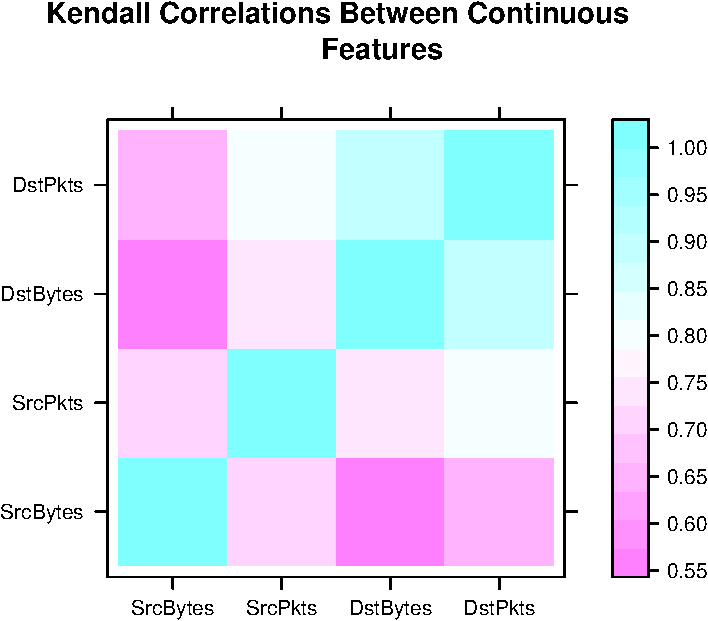
\includegraphics{thesis_files/figure-latex/unnamed-chunk-2-1.pdf}

The above matrix represents the missingness in the port combinations for
pairings of the top 20 most used source ports and destination ports. The
black cells represent missingness; of the 400 cells in the matrix, 295
(73.75\%) of cells are missing observations. This single matrix slice
can be extrapolated to missingness in ports throughout the entire tensor
because the dataset is collected in a way such that either all four
continuous features are observed, or none are observed. It is important
to note that missingness is not uniform across source and destination
port combinations. In the event that an entire row or column of port
combinations is missing, the port at that respective index will need to
be discarded from the simulation procedure because all three techniques
depend on the row and column effects when simulating a value for a
missing cell.

\section{Port Connections}\label{port-connections}

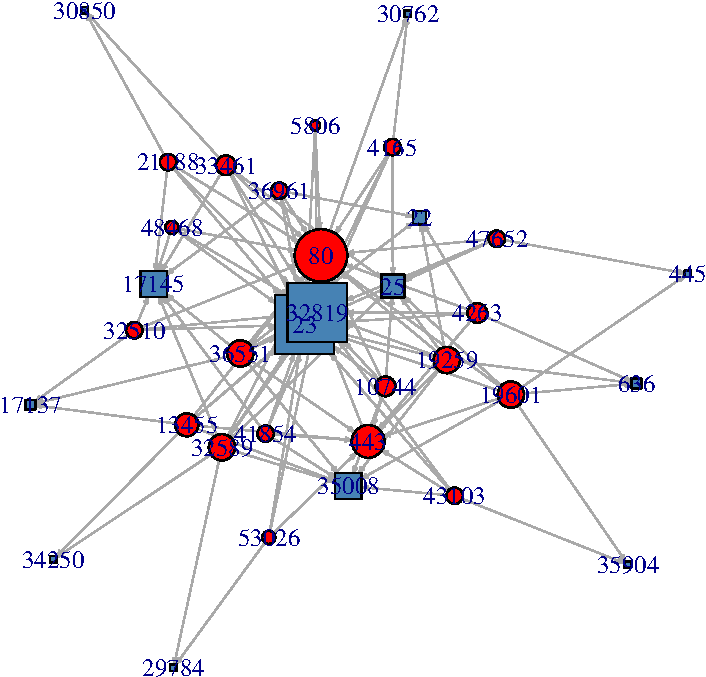
\includegraphics{thesis_files/figure-latex/unnamed-chunk-3-1.pdf}

The above ports network graph displays the pairings between the top
twenty source ports (red circles) and the top destination ports (blue
squares). When a square and circle are connected it represents that
there exist observations for this particular port combination in the
dataset. The size of each node reflects the number of paired
observations that were observed using that particular port. Clearly, not
every source port is paired with a destination port and vice versa (not
every node is connected to every other node). These missing combinations
reflect missing cells in the \(T\) tensor, and consequently they
correspond to the combinations that require values to be simulated.

\section{Varied Sample Sizes}\label{varied-sample-sizes}

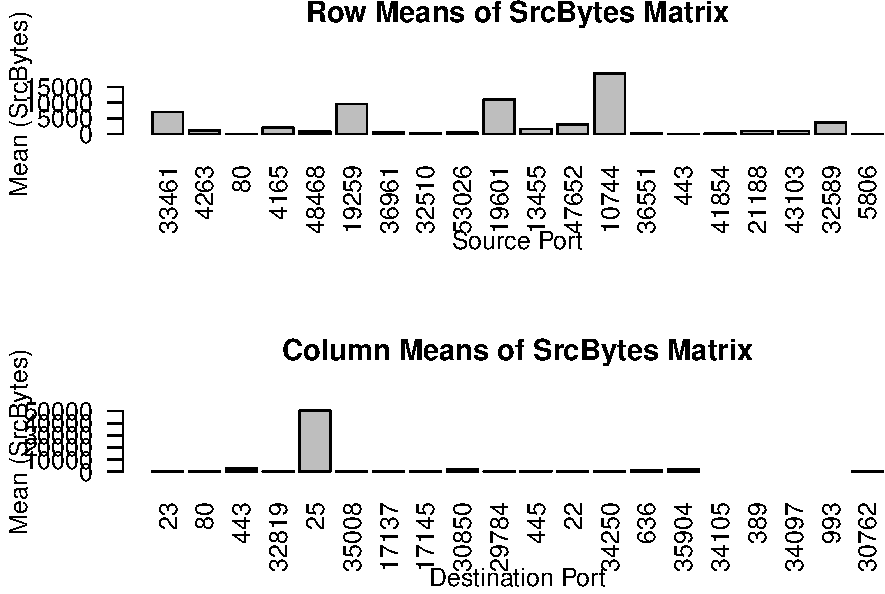
\includegraphics{thesis_files/figure-latex/unnamed-chunk-4-1.pdf}

To better visualize the sample sizes first displayed in the network
graph, the above heat plot represents the sample sizes for each
source-destination port combination on a log scale for clarity. It is
again clear there are certain combinations that have many observations
(range of 35000 on the original scale), while most of the observations
are 0, indicating no observations were observed and the corresponding
cell in \(T\) is missing, or near 0, indicating few observations were
observed. The large variation in sample sizes again suggests a
simulation technique that accounts for sample size of a missing cell's
related row and column cells is necessary.

\section{Row and Column Properties}\label{row-and-column-properties}

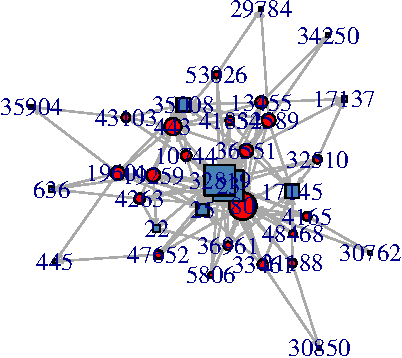
\includegraphics{thesis_files/figure-latex/unnamed-chunk-5-1.pdf}

The bar plots above represent the row and column means of the continuous
features for each slice of the tensor. These row means and column means
inform simulation techniques for the missing cells within those
respective rows and columns. There exist clear outliers in the means for
certain rows and columns. This outlier behavior is undoubtedly caused by
outliers existing within the cells in that particular row or column.
These outliers exist because each cell represents the mean of all
observations that occured within a particular port combination,
regardless of sample size (i.e.~some cells may have a few large
observations, resulting in a large mean that skews the cell's row and
column mean). Thus, cells that only have a few observed observations
have a disproportionately large effect on their respective row and
column mean.

These outliers may cause problems with simulating missing values in that
row or column because the outliers will have a disproportionately large
effect on the simulated value than the other observations, which are
more close to the median in the missing value's row or column. This
behavior suggests that the completion techniques that take into account
variances among the row and column means and the number of samples
observed for each port combination will result in more accurate
estimations for the missing port combinations.

\section{Correlations}\label{correlations}

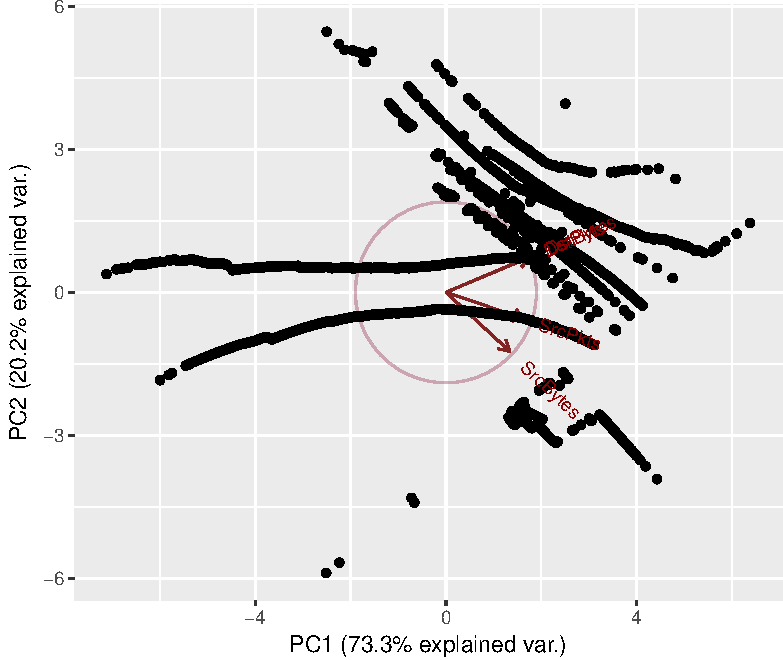
\includegraphics{thesis_files/figure-latex/unnamed-chunk-6-1.pdf}

The matrix above describes the Kendall rank correlations (commonly
referred to as Kendall's tau coefficent) between the four continuous
features in the dataset. Intuitively, the Kendall correlation between
two features will be high when observations have a similar rank
(i.e.~relative position label of observations within the variable: 1st,
2nd, 3rd, etc.) between the two variables, and low when observations
have a dissimilar rank between the two variables. The range of
correlations is {[}-1, 1{]}. Kendall correlation was selected as a
measure because it evaluates ranks between observations, as opposed to
Pearson, which is more susceptible to outliers in the dataset (large
byte and packet observations in the continuous features skewed the
Pearson measures).

It is clear there exist strong correlations between the four continuous
features, DstBytes and DstPkts in particular. This behavior suggests a
technique that simulates estimates for the missing cells with all four
features considered at once (i.e.~a technique that simulates the entire
tensor as a whole rather than in slices) will also be valuable.

Additional data analysis, including principal component analysis of the
cells and the exploration of the different scale transformations, can be
found in the Appendix.

\chapter{Alternating Least Squares Applied to Two Dimensional
Matrices}\label{alternating-least-squares-applied-to-two-dimensional-matrices}

This approach determines the best low-rank approximation for \(Y\) using
the Eckart-Young-Mirsky Theorem to repeatedly generate the orthonormal
matrices \(U\) and \(V\) of the singular value decomposition of \(Y\)
(\(Y = UDV^T\)) in an alternating pattern. The technique is proven to
correctly determine a low rank approximation on simulated matrices where
the true rank is known. Once the optimal low rank is determined from the
actual dataset the optimal low rank is used in the technique to simulate
the estimates for the missing cells of \(Y\). The technique's fit is
assessed by comparing the fitted versus the observed values

\section{Related Work}\label{related-work}

A common approach to matrix completion revolves around the underlying
assumption that there exists a low rank approximation for the data
matrix, particularly in the case of high dimensional data. Hastie,
Mazumder, Lee, and Zadeh (2014) devised a similar approach to the one
presented in this chapter that fuses nuclear-norm-regularized matrix
approximation (Candes and Tao, 2009, Mazumder, Hastie and Tibshirani,
2010) and maximum-margin matrix factorization (Srebro, Rennie and
Jaakkola, 2005), resulting in a fast alternating least squares that
relies on a low rank singular value decomposition to drive an efficient
algorithm for large matrix factorization.

Similar techniques for matrix completion were employed heavily in the
Netflix Challenge where competitors predicted ratings for movies by
users that had not watched the movie based on the other ratings in the
matrix of users and movies. The winning team, BellKor's Pragmatic Chaos,
employed a low rank decomposition technique to reduce the incredibly
large dataset, so that other algorithms could be applied without too
much computational overhead (Andreas Toscher, Michael Jahrer, Robert M.
Bell 2009).

Network datasets can range up to billions of observations (recall this
particular dataset with 1 million observations was collected in just
five minutes). Furthermore, there are up to 65000 possible network
source and destination ports, so the resulting network tensor has large
dimensions. Given the nature of the dataset and prior work in matrix
completion, the technique in this chapter assumes a low rank
decomposition to implement an alternating least squares completion
technique.

\section{Matrix Completion Algorithm}\label{matrix-completion-algorithm}

\(F \in \mathbb{R}^{m \times n}\) is a sparse matrix that represents the
frequencies of combinations, i.e \(F[32242,12312]\) represents the
number of observations for the 32242 12312 port combination
\(M \in \mathbb{R}^{m \times n}\) represents a boolean matrix of whether
the corresponding \(Y\) values are missing. \(Y[M]\) represents all of
the missing values in \(Y\).

The objective is
\[\underset{r}{\text{min}} \sum_{i,j:F_{i,j} > 0} (y_{i,j} - u_iDv^T_j)^2\]
where \(UDV^{(k)T}\) represents the singular value decomposition of
\(Y\) and \(r\) is the low rank approximation for \(Y\). There are
multiple steps to the matrix completion process:

\subsection{ANOVA Initial Imputation}\label{anova-initial-imputation}

An analysis of variance (ANOVA) imputation is used to fill in the
initial values for \(y_{ij}\). This yields an additive model dependent
upon the means of the present observations:
\[y_{ij} =  a_i + b_j - \mu\] where\(\mu\) is the overall mean of \(Y\),
\(a_i\) is the row mean, and \(b_j\) is column mean of \(y_{ij}\).

\subsection{Repeated Simulation}\label{repeated-simulation}

The repeated imputation procedure solves
\(Y^{(s)}[M] = R_r(Y^{(s-1)})[M]\) where \(R_r( ... )\) is the best rank
\(r\) approximation for the \(s\)-th step. For each step \((s)\) the
singular value decomposition decomposes
\[Y^{(s)} =  U^{(s)}D^{(s)}V^{T(s)}\] where \(D\) is a diagonal matrix
of the singular values, \(U\) is the left singular vectors of \(Y\) and
\(V\) is the right singular vectors of \(Y\).

The Eckart-Young-Mirsky Theorem provides the best rank \(r\)
approximation for the missing values in \(Y^{(s+1)}\). Recall \(Y[M]\)
represents all of the missing values of \(Y\). Applying the EYM theorem:
\[Y^{(s+1)}[M] = (U[,1:r]^{(s)}D[,1:r]^{(s)}V[,1:r]^{T(s)})[M]\] Where
\(U[,1:r]\) represents the first \(r\) columns of \(U\) and the same for
\(D\) and \(V\).

\subsection{Convergence Criterion}\label{convergence-criterion}

The Eckart-Young-Mirsky rank approximation step is repeated until the
relative difference between \(Y^{(s+1)}\) and \(Y^{(s)}\) falls below a
set threshold, \(H\). The relative difference threshold is expressed:
\[\frac{\|Y^{(s+1)}-Y^{(s)}\|_2}{\|Y^{(s)}\|_2} < H\] where \(\|Y\|_2\)
is the Frobenius norm for matrices. The denominator of the expression
ensures the convergence criterion is invariate to a scale change in the
matrix itself.

\section{Best Low Rank Approximation}\label{best-low-rank-approximation}

To determine the best low rank for approximating \(Y\), Leave-One-Out
Cross Validation (LOOCV) is used to generate prediction errors for each
possible rank. LOOCV cycles through the observed values, setting each to
NA (missing), and then performing the described matrix completion
process. The prediction error is then calculated as some function of the
difference between the imputed value and the true value. In this case,
the algorithm records root mean square error
\[\sqrt{\frac{\sum (\hat y_{ij} - y_{ij})^2}{z}}\] where \(z\) is the
number of observations not missing.

\section{Validation Against Simulated
Data}\label{validation-against-simulated-data}

Before applying the algorithm on the real data it is useful to validate
the algorithmic approach against simulated data where the true rank is
already known.

\subsection{Simulating a Low Rank
Matrix}\label{simulating-a-low-rank-matrix}

Taking the Kronecker product of two lower dimension matrices yields a
higher dimension matrix with low rank. Explicitly, given matrix
\(A \in \mathbb{R}^{m \times r}\) and \(B \in \mathbb{R}^{r \times n}\),
\(A \otimes B = C\) where \(C \in \mathbb{R}^{m \times n}\) has rank
\(r\). Thus, when \(r < m, r < n\) the matrix \(C\) has an optimal low
rank that minimizes the root mean square error from the leave one out
cross validation procedure. To add noise to the simulated matrix, \(C\),
simply add an error matrix, \(E \in \mathbb{R}^{m \times n}\) sampled
from a normal distribution.

This procedure provides a computationally efficient way to simulate many
random low rank matrices to use as inputs for the validation procedure.
In the case of simulated matrices, there are no missing entries, so the
leave one out cross validation procedure sequentially removes each cell
in the matrix, imputes its value using the rank being investigated, and
considers the individual cell error as the difference between the true
value and the imputed value. The overall root mean square error for the
technique is then calculated with the aggregate each of these individual
cell errors.

\subsection{Approximating Optimal
Rank}\label{approximating-optimal-rank}

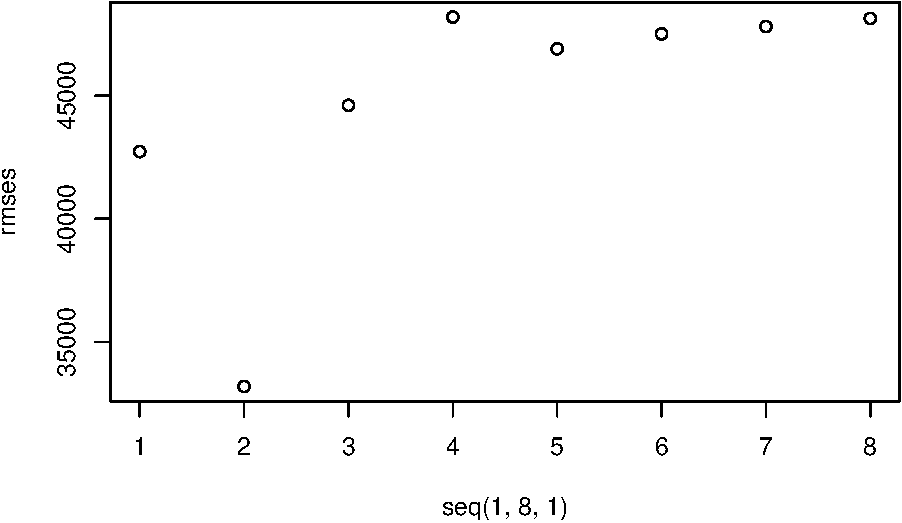
\includegraphics{thesis_files/figure-latex/unnamed-chunk-11-1.pdf}

The above plots represent the accuracy of the matrix completion
technique for matrices with true rank \(r = 1,2,...8\). The accuracy is
measured by simulating 10 random matrices (dimensions ranging from 74 to
100 values) with low rank of \(r\) for each value of \(r\) (80 simulated
matrices total), and then running the leave one out cross validation
procedure described above on the matrix \(C\) to generate a root mean
square error for each possible rank. The accuracy is the calculated
using the number of times the rank with the lowest error matches the
true simulated rank divided by 100 (the number of trials with rank
\(r\)). Note as the true rank becomes larger, the technique performs far
worse at determining the true rank. This behavior is due to the fact
that LOOCV attempts to find the rank that minimizes the root mean square
error, not necessarily the true low rank approximation for a matrix.
Higher true ranks tend to give higher out-of-sample validation error, so
LOOCV will still select a low rank approximation for simulated matrices
that have relatively high true ranks. For instance, a simulated data
matrix may have a true rank of 8, but it may also be very close to rank
2, which results in LOOCV selecting rank 2 as the optimal low rank
approximation for minimizing error.

Furthermore, when noise is applied to each simulated matrix, \(C\),
(through the addition of a noise matrix \(E\)), the algorithm tends to
perform worse at a majority of the attempted ranks. This is expected
because the addition of noise to every cell in the matrix may obscure
the true rank from the LOOCV procedure.

\section{Results on Real Data}\label{results-on-real-data}

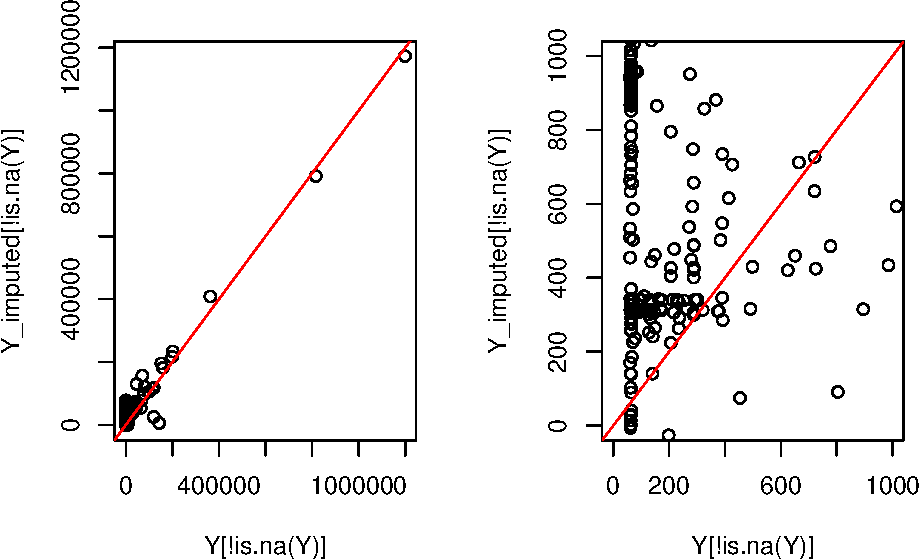
\includegraphics{thesis_files/figure-latex/unnamed-chunk-12-1.pdf}

The above plot displays the root mean square errors from the leave one
out cross validation process across different rank inputs into the
algorithm. It's clear that rank 2 provides the best low-rank
approximation for simulating missing values in \(Y\) using the
alternating least squares algorithm. Thus, the dataset is fitted with
the algorithm using rank 2 to simulate the missing values in \(Y\).

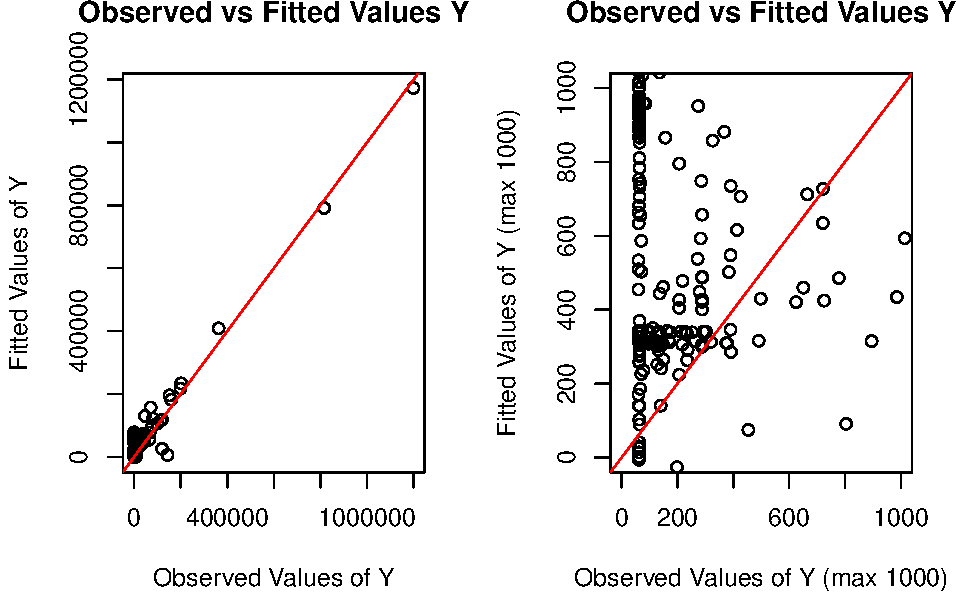
\includegraphics{thesis_files/figure-latex/unnamed-chunk-13-1.pdf}

The two plots above display the true values of the \(Y\) matrix
(i.e.~the non-missing values) versus their corresponding fitted values
using the alternating least squares algorithm with an input of rank 2.
The first plot displays all values and shows a somewhat positive linear
trend (an ideal fit of the true values would be a scatter of points
following a linear relationship, represented in red). However, several
outliers with large true values skew this dataset and cause the plot to
appear linear. Closer examination of the true and fitted values smaller
than 1000 (the plot on the right) reveals the relationship is far from
the linear pattern.

\subsection{Scale Transformations}\label{scale-transformations}

The poorly fitted results motivates a consideration of the scale of the
data. The present algorithm uses the sample averages of the overall
matrix as well as the row and column means when imputing each missing
cell value. This reliance upon sample means leads to susceptiblity to
outliers. Moreover exploratory data analysis reveals the dataset
contains outliers, particularly in the SrcBytes and DstBytes
measurements. Because outliers drive the sum of squares for the
alternating least squares procedure, the poor fit on the data is
unsurprising. Thus, a transformation of features in the dataset may be
appropriate for improving the fit of the algorithm.

When a natural logarithm transformation is applied to the raw dataset
before any simulation steps are taken, the alternating least squares
imputation algorithm yields the following root mean square errors varied
by rank.

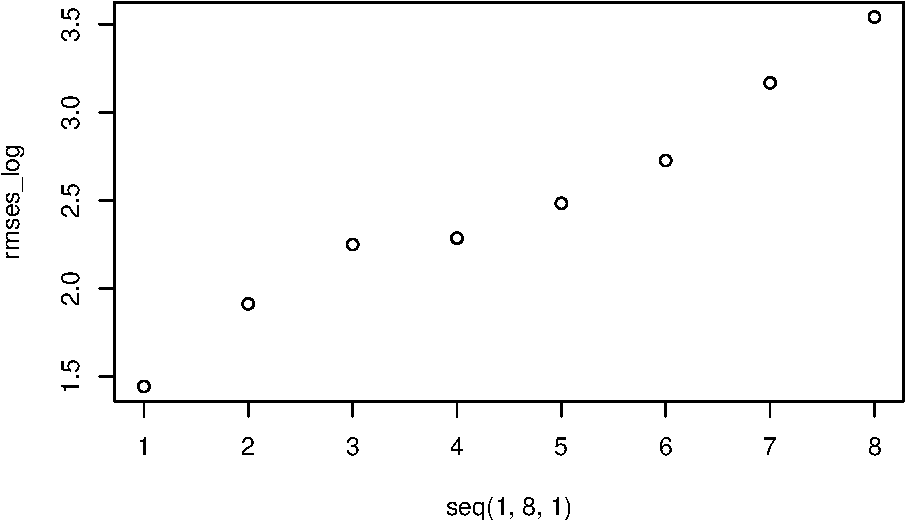
\includegraphics{thesis_files/figure-latex/unnamed-chunk-14-1.pdf}

Now the optimal rank from the LOOCV procedure is 1. The algorithm is run
on the log transformed dataset with a low rank approximation of 1 and
the fitted vereus observed values are again compared.

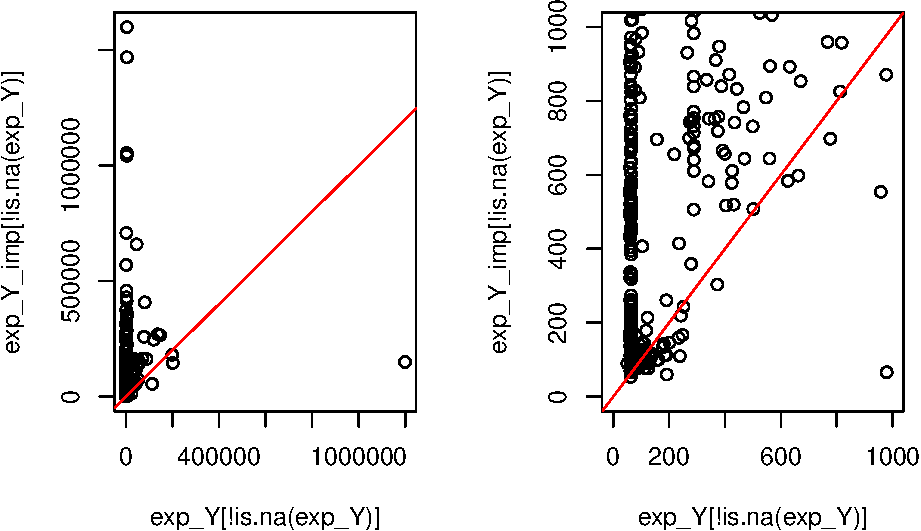
\includegraphics{thesis_files/figure-latex/unnamed-chunk-15-1.pdf}

The values above have been retransformed (exponentiated) to the
dataset's original scale after the simulation procedure was completed.
The fit still appears to be quite poor and there is not much difference
between the log transformed output versus the original non-transformed
output.

This poor performance may largely be due to the fact the algorithm does
not account for the variability in the sample size and variance in the
observed interactions for each cell. Unlike the Netflix Competition, in
which each cell of the matrix being completed contained only a single
user rating of a movie, the matrix in this problem contains the mean of
a variable number of observations corresponding to particular port
combinations.

\chapter{A Bayesian Approach to Two Dimensional Matrix
Completion}\label{a-bayesian-approach-to-two-dimensional-matrix-completion}

The previous section's results reflected the need for a completion
strategy that accounts for the variability in the number of observations
observed for each port combination when imputing that particular
combination's cell. The previous technique fails to take into account
the differing sample size and variance in each cell's observations, so
the algorithm treated each \(y_{ij}\) as a single value rather than the
mean and variance of a vector of observations. The following section
constructs a statistical model that takes the sample size of
observations and their variances for each cell into account and
repeatedly simulates values for the missing cells using a Gibbs Sampling
procedure. The sampling procedure relies upon first building a general
model for simulating the row and column facors with their respective
standard deviations. After calculating the full conditionals for the
parameters of this general model, the overall procedure repeatedly
simulates values from these full conditional distributions, alternating
between simulating the matrix of row factors and the matrix of column
factors along with their respective standard deviations. Note, this
technique again slices the tensor into the four separate matrices,
\(Y^{(1)}, Y^{(2)}, Y^{(3)}, Y^{(4)} \in \mathbb{R}^{m \times n}\)
(referred to as \(Y\) in general), and the model can be applied to each
matrix \(Y^{(k)}\) separately.

\section{Related Work}\label{related-work-1}

Bayesian methods are becoming increasingly popular as a matrix
completion technique for large scale datasets. Work by Zhou, Wang, Chen,
Paisley, Dunson and Carin (2010) indicate Gibbs Sampling provides an
efficient solution to large scale problems and yields ``predictions as
well as a measure of confidence in each prediction.'' Their paper
considers algorithm performance in several datasets of varying scale and
relationship between variables, and the results indicate strong
performance compared to other common approaches. Granted, this approach
considers non-parametric Bayesian matrix completion, while the Gibbs
Sampler in this chapter relies upon constructing the full conditional
distributions for parameters in a defined statistical model.
Nevertheless, the hypothesis remains that Gibbs Sampling provides an
efficient and effective solution for matrix completion. Mai and Alquier
also support this claim in their paper ``A Bayesian Approach for Noisy
Matrix Completion: Optimal Rate under General Sampling Distribution''
(2014), in which they construct a Bayesian estimator that relies upon
the premise that ``Bayesian methods for low-rank matrix completion with
noise have been shown to be very efficient computationally.'' They apply
this technique to the Netflix competition dataset as a case study.

\section{Statistical Model for Port
Relationships}\label{statistical-model-for-port-relationships}

The following statistical model is defined for the cells in \(Y\):
\[y_{ij} = u_i^Tv_j + \frac{\sigma_i \tau_j}{\sqrt{s_{ij}}}\epsilon_{ij}\]
where \(u_i\) represents the row factors, \(v_j\) represents the column
factors, \(\sigma_i\) represents the standard deviation of each row in
the matrix, \(\tau_j\) represents the standard deviations of each column
in the matrix, \(s_{ij}\) represents the sample size of observations
observed for source port \(i\) and destination port \(j\), and
\(\epsilon_{ij} \sim N(0,1)\). Fixing the \(j\) values in the analysis
(i.e. \(v_j\) and \(\tau_j\) are known) enables the model to be
rewritten in the form of a weighted least squares model for imputing
\(u_i\) and \(\sigma_i\). Similarly, when \(i\) is fixed, the model can
be rewritten to simulate \(v_j\) and \(\tau_j\). To demonstrate this
property, the procedure for simulating \(u_i\) and \(\tau_j\) given
known values for \(v_j\) and \(\tau_j\) is described below. The same
procedure is possible for \(v_j\) and \(\tau_j\) when \(u_i\) and
\(\sigma_i\) are known.

\section{General Model for Simulating Row and Column
Factors}\label{general-model-for-simulating-row-and-column-factors}

Varying \(j = 1 ... n\) the model above yields the following cell
values:
\[y_{i1} = u_i^Tv_1 + \frac{\sigma_1 \tau_j}{\sqrt{s_{ij}}}\epsilon_{ij}\]
\[ ... \]

\[ y_{in} = u_i^Tv_n + \frac{\sigma_i \tau_j}{\sqrt{s_{ij}}}\epsilon_{ij} \]

Vectorizing all of these equations varied across \(j = 1...n\) yields:

\[\vec{y_i} = Vu_i + \sigma_i W^{1/2}\vec{\epsilon}\]

where \(V \in \mathbb{R}^{n \times r}\) is the matrix of column factors
(\(p\) is the dimension of the latent factors), and
\(W \in \mathbb{R}^{n \times n}\) is the diagonal matrix of weights,
such that \[V =
  \begin{bmatrix}
    v_1^T- \\
    v_2^T- \\
    ... \\
    v_n^T- \\
  \end{bmatrix},
  W =
  \begin{bmatrix}
    w_{1} & & \\
    & \ddots & \\
    & & w_{n}
  \end{bmatrix} 
  = \begin{bmatrix}
    \frac{\tau_1^2}{s_{11}} & & \\
    & \ddots & \\
    & & \frac{\tau_n^2}{s_{nn}}
  \end{bmatrix}\]
Note \(\tau^2\) refers to the variance, variance being the square of the
standard deviation.

This model can be rewritten in a general form:

\[\vec{y} = X\beta + \sigma W^{1/2}\epsilon\] where \(X\) represents
\(V\), \(\beta\) represents \(u_i\) and \(sigma\) represents
\(\sigma_i\).

This is a modified form of the Generalized Least Squares Model (GLS),
which gives a weighted least squares estimate of \(\beta\), and it is
appropriate when the error terms are not independent and identically
distributed. Bayesian analysis of this problem provides similar
parameter estimates to GLS, and both ordinary least squares and GLS
provide unbiased parameter estimates of \(\beta\) with the latter giving
estimates with a lower variance because the non-Bayes estimator serves
as a limit of the Bayes estimator.

The full conditional distributions of the random variables \(\beta\) and
\(\sigma^2\) (note \(\sigma\) is squared in the model) for this case are
described below:
\[\{\beta \mid X, \vec{y}, \sigma^2\} \sim MVN (\beta_n, \Sigma_n)\]
\[\{\sigma^2 \mid X, \vec{y}, \beta\} \sim IG (\frac{\nu_0 + n}{2}, \frac{v_0\sigma^2_0 + SSR_W}{2})\]
where MVN represents the Multivariate Normal Distribution, and IG
represents the Inverse Gamma distribution. \[ \begin{cases}
      \Sigma_n = (X^TW^{-1}X/\sigma^2+\Sigma_0^{-1})^{-1}\\
      \beta_n = \Sigma_n(X^TW^{-1}y/\sigma^2 + \Sigma_0^{-1} \beta_0)
    \end{cases}\] \[SSR_W = (y - X\beta)^TW^{-1}(y-X\beta)\]
The formulation for the closed form full conditional distributions for
the \(\beta\) and \(\sigma^2\) parameters are based upon the general
full conditionals established for a regression model with correlated
errors (Hoff 2009). These particular full conditional formulations are a
special case of this model where \(W\) is a diagonal matrix and so the
covariance matrix is diagonal. This general regression model formulation
also conveniently specifies the prior distributions.

The remaining variables in the closed form full conditionals come from
the parameter's prior distributions, which are defined as follows:

\[\beta \sim MVN (\beta_0, \Sigma_0)\]
\[\sigma^2 \sim IG (\frac{\nu_0}{2}, \frac{v_0}{2}\sigma_0^2)\]

The initial values for the prior distributions are set as:
\(\beta_0 = 0\), \(\Sigma_0 = \gamma^2I\) where \(\gamma^2\) is a large
number and \(I\) is the \(m \times n\) identity matrix, \(\nu_0 = 2\),
\(\sigma_0^2 = 1\). This results in a diffuse prior for \(\beta\) that
spreads out the density, and a noninformative prior for \(\sigma^2\).

Work by Alquier, Cottet, Chopin, Rousseau (2014) reveal that a standard
approach to assigning priors in Bayesian Matrix completion ``is to
assign an inverse gamma prior to the singular values of a certain
singular value decomposition of the matrix of interest; this prior is
conjugate. However, {[}they{]} show that two other types of priors
(again for the singular values) may be conjugate for this model: a gamma
prior, and a discrete prior. Conjugacy is very convenient, as it makes
it possible to implement either Gibbs sampling or Variational Bayes.''
In the case of this problem, the distributions of the priors are defined
to be diffuse (\(\beta\)) and noninformative (\(\sigma^2\)), so that the
effects of the priors on the posteriors are limited when compared to the
effects of the observed data.

\subsection{Generalized Gibbs Sampler
Function}\label{generalized-gibbs-sampler-function}

Following the formulation of the model and the definition of the priors,
a general Gibbs Sampler function is created to simulate samples from the
full conditional of each parameter in the statistical model, which
iteratively creates an approximate value for each cell.

The Gibbs Sampler algorithm progresses as follows:

Let the parameters at step \(s\) be:

\(\phi^{(s)} = \{\beta^{(s)}, \sigma^{2(s)}\}\)

Sample \(\beta^{(s+1)} \sim P(\beta \mid X, \vec{y}, \sigma^{2(k)})\)

Sample \(\sigma^2 \sim P(\sigma^2 \mid X, \vec{y}, \beta^{(s+1)})\)

Set \(\phi^{(s+1)} = \{\beta^{(s+1)}, \sigma^{2(k+1)}\}\)

This Gibbs Sampler serves as a general technique that can be used to
simulate both the values of \(u_i\) and \(\sigma_i\) or \(v_j\) and
\(\tau_j\) depending on the inputs it is given because the formulation
of both models are identical; they only differ by the the inputs, \(X\)
and \(W\), which are calculated, and \(y\) which is sliced directly from
\(Y\). In the context of the problem, this function can first be called
repeatedly to simulate all of the rows in the matrix \(Y\), then called
repeatedly with updated inputs to simulate all of the columns of the
matrix.

\subsection{Validation Simulated Data}\label{validation-simulated-data}

Before using the general Gibbs sampler function in the overall procedure
for simulating missing values in \(Y\), it is necessary to validate the
procedure's effectiveness on simulated data where the ground truth is
known. As the algorithm runs, it stores a matrix of \(\beta\) vectors
and a vector of \(\sigma^2\) scalars. Thus, if \(S = 50\), i.e.~the
algorithm samples 50 \(\beta\) and 50 \(\sigma\), the final returned
output will be \[\beta =
  \begin{bmatrix}
    \beta_1^T- \\
    \beta_2^T- \\
    ... \\
    \beta_{50}^T- \\
  \end{bmatrix},
  \vec{\sigma^2} =
  \begin{bmatrix}
    \sigma_1^2 \\
    . \\
    . \\
    \sigma_{50}^2\\
  \end{bmatrix}\]
Using random sampled values from the normal distribution for \(X\) and
random sampled values from the exponential distribution for \(W\)
(exponential distribution is used to ensure \(\Sigma_n\) is positive
definite), it is possible to calculate values of \(\vec{y}\) using a
predefined \(\beta*\) and \(\sigma *\), which are known as the ground
truth values for comparison:
\[\vec{y} = X\beta * + \sigma * W^{1/2}\epsilon\] This \(\vec{y}\),
\(W\), and \(X\) are used as inputs to the general Gibbs Sampler
Function to generate a distribution of \(\beta\)'s and a distribution
\(\sigma^2\)'s. The posterior means of these distributions are then
computed and compared to recover the original values, \(\beta *\) and
\(\sigma *\).

In particular, the posterior mean of \(\sigma^2\) is calculated by
taking the mean of the function's output of \(\sigma^2\). This posterior
mean is compared to the original \(\sigma *\) used to generate
\(\vec{y}\). Repeatedly performing this procedure reveals the posterior
mean only differs from the ground truth value by 1-2\% in almost every
single trial.

Recovering the original \(\beta *\) provides a much more defined
procedure for evaluating the performance of the Gibbs Sampler. First,
the Bayes estimator (the posterior mean of generated \(\beta\)s) should
be close to the GLS estimator and theoretical results state the GLS
estimator serves as a good approximation for the true value.
Furthermore, the variance matrix of the GLS estimator around the true
value is
\[Var(\hat{\beta}_{GLS}) = \mathbb{E}[(\hat{\beta}_{GLS}-\beta * )(\hat{\beta}_{GLS}-\beta *)^T]=(X^T W^{-1}X/\sigma^2 )^{-1}\].
Thus, after simulating many data sets and solving for the posterior mean
estimator, \(\hat{\beta}\), the variance of these simulated posterior
means, \(Var(\hat{\beta})\) should be close to
\((X^T W^{-1}X/\sigma^2 )^{-1}\). Moreover, the standard errors are
calculated
\[SE(\hat{\beta}_{GLS}) = \sqrt{diag((X^T W^{-1}X/\sigma^2 )^{-1})}\].
This provides a nominal 95\% confidence interval for which to assess the
performance of the model for recovering the original \(\beta *\).

\section{Full Sampling Procedure}\label{full-sampling-procedure}

The complete sampling procedure for imputing missing values uses the
generalized Gibbs Sampler defined above to iteratively simulate missing
values for the entire matrix \(Y\). The procedure is described below:

Initialize \(\sigma_i\) for \(i = 1 ... m\) and \(\tau_j\) for
\(j = 1 ... n\) as the overall standard deviation of the \(Y^{(k)}\)
matrix. Initialize missing values of \(Y\) using the ANOVA imputation
described in the previous section. Initialize the matrix of row factors
\(U \in \mathbb{R}^{m \times p}\) and the matrix of column factors
\(V \in \mathbb{R}^{n \times p}\).

Repeat the following:
\begin{enumerate}
\def\labelenumi{\arabic{enumi}.}
\item
  For \(i = 1 ... m\): Simulate \(u_i\) and \(\sigma_i\) using the
  generalized Gibbs Sampler. For the first iteration of the sampler, set
  \(X\) to the \(V\) matrix in the singular value decomposition of
  \(Y\). For all future iterations, the use the stored \(V\) from the
  pervious iteration as \(X\). For the first iteration, use the
  initialized \(\tau_j\) for \(j = 1 ... n\) to calculate the diagonals
  for the \(W\) matrix. For all future iterations use the stored
  \(\tau_j\) values from the previous iteratioWn to calculate \(W\).
  Take the corresponding \(y_i\) directly from the \(Y\) matrix. Store
  the resulting sampled \(u_i\)'s in a matrix \(U\), and the
  \(\sigma_i\) in a vector, to use for simulating \(v_j\) and
  \(\tau_j\).
\item
  For \(j = 1 ... n\): Simulate \(v_j\) and \(\tau_j\) using the
  generalized Gibbs Sampler. Use the stored \(U\) from the previous step
  as the \(X\) input and use the stored \(\tau_j\) to calculate the
  \(W\) input. Take the corresponding \(y_j\) directly from the \(Y\)
  matrix. Store the resulting sampled \(v_j\)'s in a matrix \(V\), and
  the \(\tau_j\) in a vector, to use for simulating \(u_i\) and
  \(\sigma_j\).
\item
  Simulate values for \(y_{ij}\) in \(Y\) that were missing in the
  original dataset by sampling from the normal distribution
  \[y_{ij} \sim N(u_i^Tv_j, \frac{\sigma_i^2\tau_j^2}{s_{ij}})\]
\end{enumerate}
\subsection{Selecting the Dimension of Latent
Factors}\label{selecting-the-dimension-of-latent-factors}

The dimension of the latent factors, \(p\), is used to define the
dimension of \(\beta \in \mathbb{R}^{p \times 1}\) and consequently
defines the dimensions of the row and column factor matrices \(U\) and
\(V\). Selecting \(p\) is a model selection choice similar to
determining the optimal low rank approximation \(r\) in the previous
section. Once again, Leave One Out Cross Validation may be used to
detemine the optimal \(p\) given the observed data. In this technique,
it is more computationally expensive than the previous technique to
perform Leave One Out Cross Validation on the entire dataset, so K-Fold
cross validation or randomly selecting a set number of observed cells to
set to missing for determining \(p\) is also valid.

\subsection{Validation on Simulated
Data}\label{validation-on-simulated-data}

Again it is necessary to validate the effectiveness of the overall
sampling procedure with simulated data where the ground truth is known.
Simulate matrices \(U\) and \(V\) such that \(\Theta = UV^T\) is truly
low rank. The same procedure for generating low rank matrices used in
the previous chapter can be applied here. Using \(\Theta\) there are two
possible tests for determining the validity of the sampling procedure.
First, the simulated data is used to recover the true values for
\(UV^T\) from the model. This is considered an idealized case for
testing the procedure. Second, some cells are set to missing and again
the procedure is used to obtain an estimate for \(UV^T\) from the model.
This output is compared to the previous case's output to evaluate the
performance depending on whether the cells have data or do not.

\chapter{Tensor Completion}\label{tensor-completion}

Recall the analysis of correlations between the continuous features in
\(T\) in chapter 2.

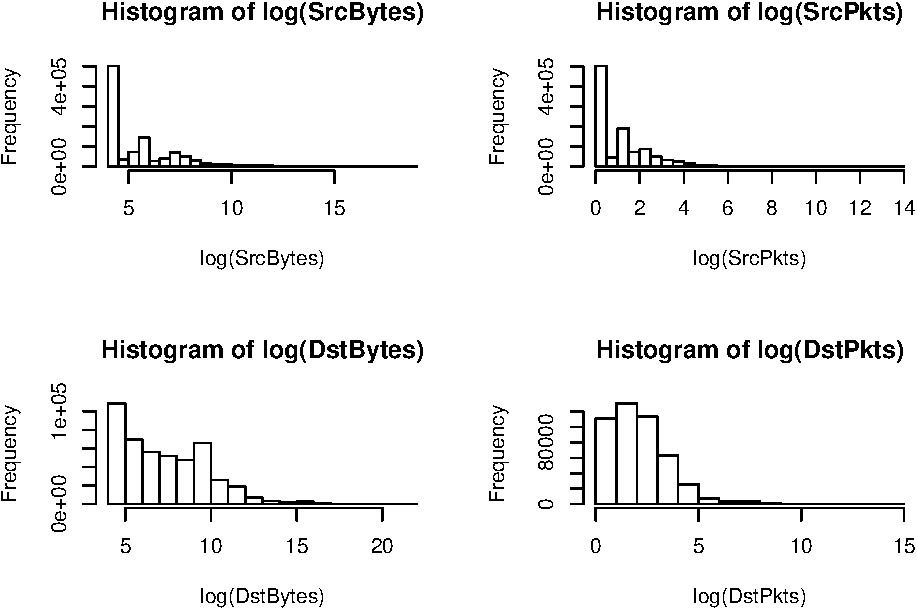
\includegraphics{thesis_files/figure-latex/unnamed-chunk-17-1.pdf}

The strong correlations between the individual continuous features
suggests imputing the tensor \(T\) all at once may yield closer
estimates than the previous two techniques, which sliced the matrices.
By imputing the tensor as a whole, techniques that include effects that
capture the relationships between features can take advantage of
possible collinearity between the features.

The following section describes the way techniques in the previous
sections may be extended to full 3-dimensional tensor completion.

\section{PARAFAC Decomposition}\label{parafac-decomposition}

The PARAFAC decomposition expresses the tensor as:
\[T = \sum_{r=1}^Ru_r \cdotp v_r \cdotp w_r\] where \(r\) represents the
rank approximation, \(\cdotp\) denotes the outer product of tensors, and
\(U \in \mathbb{R}^{m \times r}\), \(V \in \mathbb{R}^{n \times r}\),
and \(W \in \mathbb{R}^{4 \times r}\). Each individual cell is
expressed: \[t_{ijk} = \sum_{r=1}^RU_{ri} \cdotp V_{ri} \cdotp W_{ri}\]
Applying this decomposition yields the objective
\[\underset{T'} {\text{min}}\|T-T'\|\] where
\[T' = \sum_{r=1}^R\lambda_r(u_r \cdotp v_r \cdotp w_r)\] and
\(\lambda_r\) is the regularization penalty.

\section{Statistical Model}\label{statistical-model}

The following model is proposed:
\[t_{ijk} \sim N(\mu_{ijk}, \frac{\sigma^2_{ijk}}{s_{ijk}})\] where
\(\mu_{ijk}\) is the sample mean, \(s_{ijk}\) is the sample size of
observations, and \(\sigma^2_{ijk}\) is the sample variance of
observations for source port \(i\), destination port \(j\), and
continuous feature \(k\).

Substituting these values into the Gaussian probability density function
yields the likelihood:
\[\frac{s_{ijk}}{\sigma^2_{ijk}}\sum(\bar t_{ijk} - \mu_{ijk})^2\]

Applying the PARAFAC decomposition, \(\mu_{ijk}\) is re-expressed:
\[\mu_{ijk} = \sum_{r=1}^Ra_{ir}b_{jr}c_{kr}\]

Vectorizing the inputs in the likelihood yields:
\[\sum_j\sum_k[\bar t_{ijk} - a_i^T(b_i \cdotp c_k)]\frac{n_{ijk}}{\sigma^2_{ijk}}\]
where \(a_i \in \mathbb{R}^{m \times r}\),
\(b_j \in \mathbb{R}^{n \times r}\), and
\(c_k \in \mathbb{R}^{4 \times r}\). Summing across \(j\) and \(k\) in
this case solves for the \(ith\) row slice of the tensor.

\section{Future Work}\label{future-work}

Future work will use the PARAFAC decomposition and the Gaussian
statistical model described above to extend the techniques described in
chapters 3 and 4 to completing the tensor as a whole. The PARAFAC
decomposition allows for low rank tensor completion on data with high
degrees of missingness. Recent work by Yokota, Zhao, and Cichocki (2016)
propose a ``Smooth PARAFAC Decomposition for Tensor Completion'' that
``consider `smoothness' constraints as well as low-rank approximations,
and propose an efficient algorithm for performing tensor completion that
is particularly powerful regarding visual data. The proposed method
admits significant advantages, owing to the integration of smooth
PARAFAC decomposition for incomplete tensors and the efficient selection
of models in order to minimize the tensor rank.'' The statistical model
for tensor completion mimics Chapter four's technique more closely. The
full conditionals for the parameters being estimated in the model are
constructed, and a Gibbs Sampler is created using these full
conditionals to iteratively sample the three factor variables and their
respective standard deviations described in the model. Like the previous
techniques, each of these technique's validity will first be tested on
simulated data where the ground truth is known before being applied to
the real dataset.

\chapter*{Discussion}\label{discussion}
\addcontentsline{toc}{chapter}{Discussion}

This paper has developed two techniques for matrix completion that can
then be used to complete individual slices of a tensor. The first
technique, an alternating least squares procedure relies upon the
Eckart-Young-Mirsky theorem to implement low-rank singular value
decomposition. Determining the optimal low rank is a model selection
problem that is solved using leave one out cross validation to assess
the quality of possible ranks on given datasets. The validity of this
technique is tested using simulated datasets where a true low rank is
known before it is applied to the actual dataset. Finally, the procedure
is applied to the real networks dataset and its performance is evaluated
by comparing the fitted values versus the true observed values. Upon
noticed certain trends due to outliers in the comparison, a log
transformation is conducted on the original dataset and the matrix is
once again completed. The second technique constructs a statistical
model and uses Gibbs Sampling to iteratively sample values from the
parameter's full distributions. It acknowledges the weaknesses of the
first technique by including both the sample size and the standard
deviation of the observations in each matrix cell in the model. This
model ends up being very close to a Generalized Least Squares model and
so the sampling procedure for the row and the column factors in the
matrix is validated by examining the proximity of the variance of the
\(\beta\) posterior means in many simulated datasets compared to the
variance of the GLS estimator. The paper finally also proposes a
solution to extend the two techniques to imputing the tensor iteratively
as a whole, rather than individual slices.

For the empirical results throughout this paper
\(T' \in \mathbb{R}^{100 \times 74 \times 4}\): the most used 100 source
ports and their combinations with the most used 74 destination ports are
considered. This was constructed by first taking the most used 100
source and destination ports, creating a \(100 \times 100 \times 4\)
tensor, and then removing the rows and columns where all values were
completely missing because those rows and columns would not provide row
means and column means respectively to inform the completion techniques.
All of the modeling techniques are informed by the exploratory data
analysis conducted on the original dataset prior to completion steps.

Application of these completion techniques to the networks dataset
provides a reasonable estimate for the four continuous features at every
possible port combination in the matrix. This completed tensor provides
a basis for detecting anomalies in future data. For instance, new
observations for a certain port combination that fall outside a
threshold of error for the estimated value in the tensor can be marked
as as an anomaly and the source and destination IP may be flagged for
further investigation. There are two major limitations of these
techniques:
\begin{enumerate}
\def\labelenumi{\arabic{enumi}.}
\item
  The sheer size of existing and future network data makes the
  computational efficiency of the techniques a large concern. The
  techniques would need to provide a reasonable estimate for every cell
  in a tensor that may extend up to \(65535 \times 65535 \times 4\)
  (65535 is the number of overall ports). Furthermore, billions of
  observations may eventually become available, so recalculating initial
  means and standard deviations for the observations of each cell would
  need to be done carefully and to be completed in a reasonable amount
  of time. While Gibbs Sampling and alternating least squares have both
  been shown to be very efficient and are often employed for handling
  high dimensional and large scale datasets, the potential size of the
  networks datasets that may be fed into these techniques enforce the
  absolute need for computational efficiency.
\item
  The techniques do not consider the specific domain context with which
  each port is used. For instance, in TCP protocol, port number 22 is
  Secure Shell (SSH), which is one of the most popular ports for
  everyday users. Previous domain knowledge could perhaps inform
  reasonable estimates for each port combination. Some port combinations
  may be expected to have large byte and packet transfers, while others
  may be expected to have few transfers overall. Constructing additional
  models or features that incorporate domain knowledge regarding the
  particular port combinations will be useful for improving the model's
  effectiveness in detecting anomalies.
\end{enumerate}
\appendix

\chapter{Preliminary Data
Investigation}\label{preliminary-data-investigation}

\section{Exploratory Data Analysis}\label{exploratory-data-analysis}
\begin{verbatim}
     Flgs   SrcAddr     Sport   DstAddr     Dport   SrcPkts   DstPkts 
 "factor"  "factor"  "factor"  "factor"  "factor" "integer" "integer" 
 SrcBytes  DstBytes     State 
"integer" "integer"  "factor" 
\end{verbatim}
\subsection{Continuous Features: Distributions and
Relationships}\label{continuous-features-distributions-and-relationships}

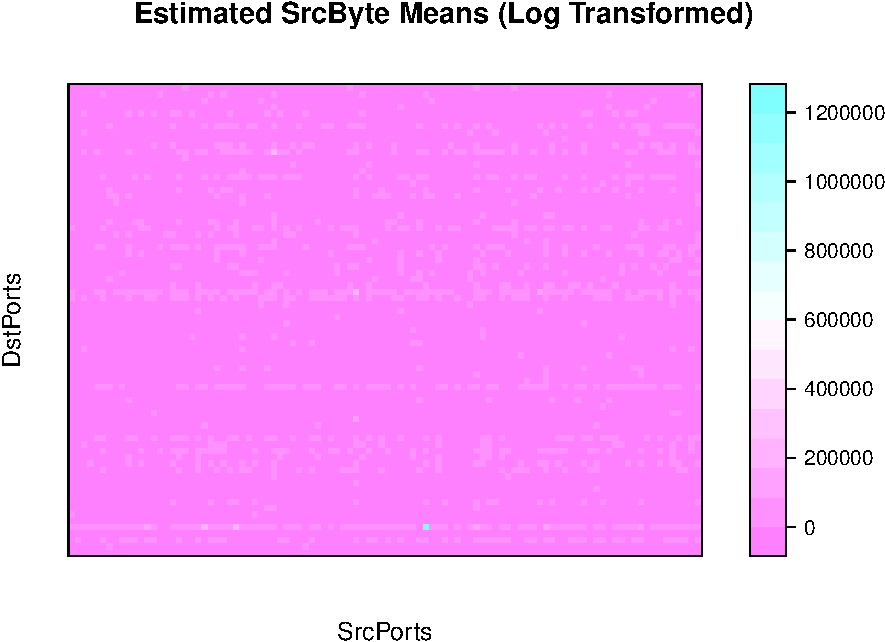
\includegraphics{thesis_files/figure-latex/unnamed-chunk-20-1.pdf}
\begin{verbatim}
 [1] 118257047 116615879 112673526 108933442 105793666  73376579  72839115
 [8]  70001807  56206409  55359912
\end{verbatim}
\begin{verbatim}
 [1] 1008233 1000971  771590  492361  458603  437296  408530  407973
 [9]  371976  371251
\end{verbatim}
\begin{verbatim}
 [1] 1850817751 1713055847 1690162763 1524781880 1491609296 1340922625
 [7] 1304668214 1206594243 1163954979 1145323438
\end{verbatim}
\begin{verbatim}
 [1] 1239611 1223485 1219276 1004471  982931  942827  883354  795120
 [9]  766776  754831
\end{verbatim}
The histograms and the largest 10 values in each of the continuous
variables show that there are a relatively few amount of large
observations skewing the distributions. This explains the model summary
containing means much larger than their medians. It's not possible to
remove the large values as outliers because they may be scanner
observations to detect. Also there is a high frequency (up to the first
quartile) of destination bytes and packets that equal 0.

We will now try to investigate whether the largest continuous predictor
values correspond to any particular addresses or ports.
\begin{verbatim}
             Flgs   SrcAddr Sport    DstAddr Dport SrcPkts DstPkts
282859  * s        1.0.12.1 18086  100.0.1.8 31743  208339  104886
282841  * s        1.0.12.1 18086  100.0.1.8 31743  204912   99688
282832  * s        1.0.12.1 18086  100.0.1.8 31743  198007   94621
282853  * s        1.0.12.1 18086  100.0.1.8 31743  191443   95892
282823  * s        1.0.12.1 18086  100.0.1.8 31743  186228   84342
724162  * *       100.0.4.9 37901 100.0.2.67    22 1008233 1239611
        SrcBytes   DstBytes State
282859 118257047    7514403   CON
282841 116615879    7146182   CON
282832 112673526    6801146   CON
282853 108933442    6857053   CON
282823 105793666    6048529   CON
724162  73376579 1713055847   CON
\end{verbatim}
\begin{verbatim}
             Flgs   SrcAddr Sport    DstAddr Dport SrcPkts DstPkts
2162    * d       197.0.1.1 62030  100.0.1.1    80  371251 1219276
724162  * *       100.0.4.9 37901 100.0.2.67    22 1008233 1239611
724106  * *       100.0.4.9 37901 100.0.2.67    22 1000971 1223485
2212    * d       197.0.1.1 62034  100.0.1.1    80  280593 1004471
78245   * d         1.0.2.1 11210  100.0.1.2    80  158194  982931
2185    * d       197.0.1.1 62033  100.0.1.1    80  268402  883354
       SrcBytes   DstBytes State
2162   26430322 1850817751   CON
724162 73376579 1713055847   CON
724106 72839115 1690162763   CON
2212   20037592 1524781880   FIN
78245  11294111 1491609296   CON
2185   19137354 1340922625   FIN
\end{verbatim}
Source Addresses tend to be repetitive for the largest max
bytes/packets, while ports vary. The top 10 largest DstBytes all
correspond to SrcAddr 197.0.1.1 and DstAddr 100.0.1.1. Also both max Src
and Dst rows correspond to the ``* s''" flag. The largest sizes of
DstBytes tend to go to Dport 80, which is the port that expects to
receive from a web client (http), while the largest SrcBytes go to
31743. The next section implements a systematic way for investigating
the relationship between addresses and ports because simply looking at
the max rows is difficult.

\section{Transformations on the Data}\label{transformations-on-the-data}

\subsection{Removing Quantiles}\label{removing-quantiles}

To get a better sense of the unskewed distribution, the below plots
visualize the continuous features with the largest and smallest 10\% of
observations removed. The removed values will be readded to the dataset
when investigating for anomalies.

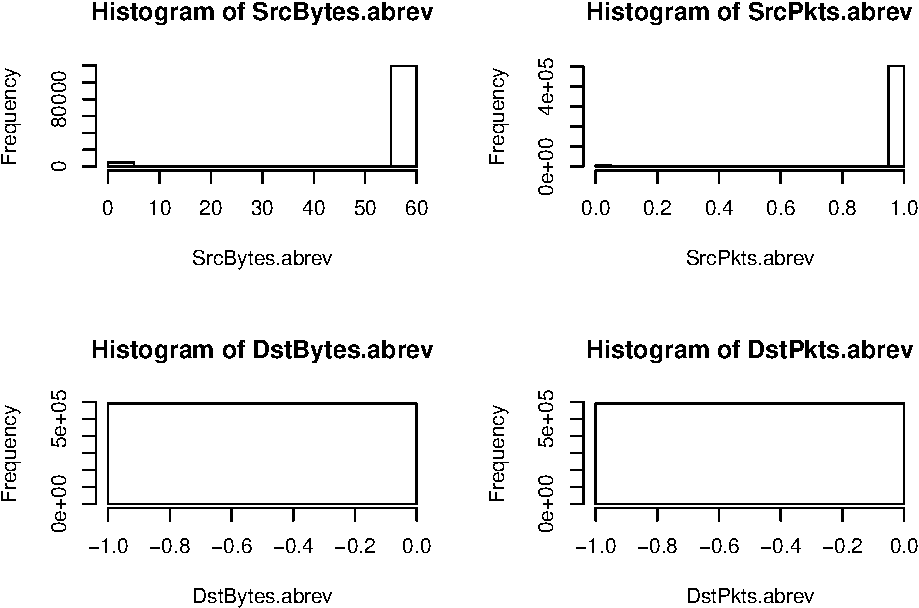
\includegraphics{thesis_files/figure-latex/unnamed-chunk-22-1.pdf}

The continuous features are still unevenly distributed even with the
20\% most extreme values removed.

\subsection{Log Transformation}\label{log-transformation}

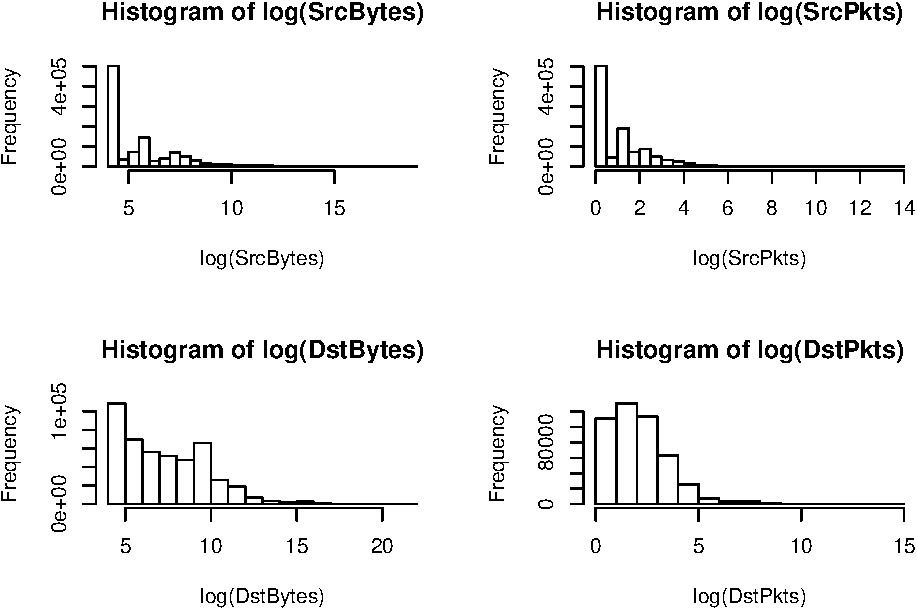
\includegraphics{thesis_files/figure-latex/unnamed-chunk-23-1.pdf}
\includegraphics{thesis_files/figure-latex/unnamed-chunk-23-2.pdf}

A log transformation for each of the continuous features outputs
right-skewed histograms. Skewed features may affect the results of a
kernel pca, so we consider other approaches for transformations.

\subsection{Normal Scores
Transformation}\label{normal-scores-transformation}

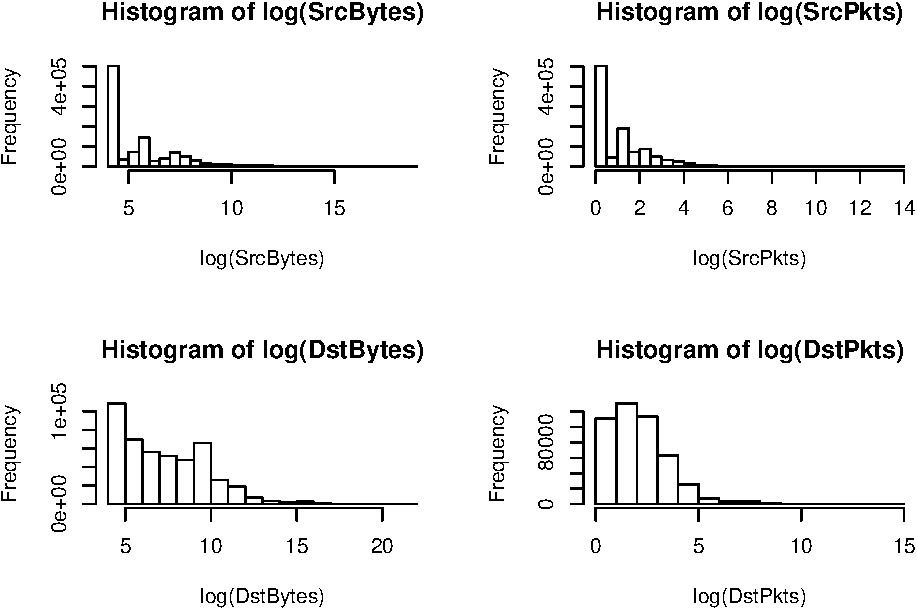
\includegraphics{thesis_files/figure-latex/unnamed-chunk-24-1.pdf}

Finally, a normal scores transformation is applied to the dataset. The
normal scores transformation reassigns each feature value so that it
appears the overall data for that feature had arisen or been observed
from a standard normal distribution. This transformation solves the
issue of skewness-each value's histogram will now follow a standard
gaussian density plot-, but it may cause issues with other analysis
methods, particularly methods that are susceptible to ties in data.

\section{Principal Component
Analysis}\label{principal-component-analysis}

Principal component analysis represents data in terms of its principal
components rather than relying on traditional Cartesian axes. Principal
components contain the underlying structure in data by representing the
directions that contain the most variance. Each successive principal
component is orthoganol to the previous, so the resulting vectors yields
an uncorrelated orthogonal basis set. Because PCA is sensitive to
relative scaling of variables, a normal scores transformation is applied
before the algorithm is run.

\subsection{Application}\label{application}

In this problem, Principal Component Anaylsis is applied to each
source-destination port grouping of observed data to understand the
underlying structure of the data partition's continuous features: source
bytes and packets and destination bytes and packets. In particular the
amount of variance explained by the generated principal components and
their relative directions will signal whether specific trends in
connection behavior occur at certain ports, and whether the size of each
of the continuous features affects port behavior as well as the other
features.

\section{Implementation}\label{implementation}

\subsection{Investigating Port
Combinations}\label{investigating-port-combinations}
\begin{verbatim}
Sport: 32416    Dport: 9163 
               PC1        PC2        PC3          PC4
SrcBytes 0.4113308 -0.7246604 -0.5528760  0.001575730
SrcPkts  0.5054262 -0.3234250  0.7999554  0.003459252
DstBytes 0.5357591  0.4327433 -0.1665939  0.705649994
DstPkts  0.5369483  0.4277813 -0.1632360 -0.708550377
Importance of components:
                          PC1    PC2     PC3     PC4
Standard deviation     1.7118 0.8991 0.51065 0.02309
Proportion of Variance 0.7326 0.2021 0.06519 0.00013
Cumulative Proportion  0.7326 0.9347 0.99987 1.00000
\end{verbatim}
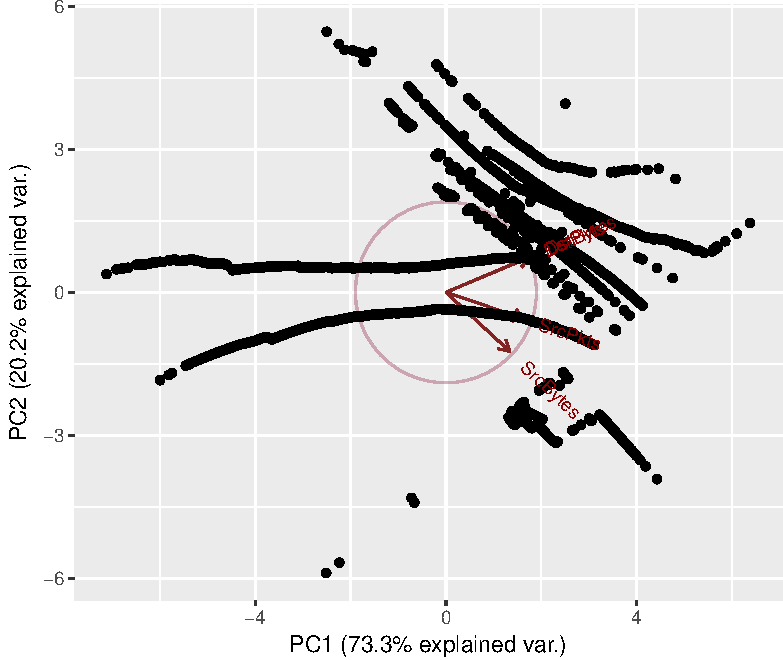
\includegraphics{thesis_files/figure-latex/unnamed-chunk-26-1.pdf}
\begin{verbatim}
Sport: 4145     Dport: 9119 
               PC1        PC2        PC3          PC4
SrcBytes 0.4333309  0.8902089 -0.1405308  0.001886624
SrcPkts  0.5213529 -0.1206221  0.8439979  0.036180840
DstBytes 0.5190742 -0.3165495 -0.3953966  0.688490995
DstPkts  0.5205549 -0.3045896 -0.3340362 -0.724339380
Importance of components:
                         PC1    PC2     PC3     PC4
Standard deviation     1.875 0.6538 0.23124 0.05551
Proportion of Variance 0.879 0.1069 0.01337 0.00077
Cumulative Proportion  0.879 0.9859 0.99923 1.00000
\end{verbatim}
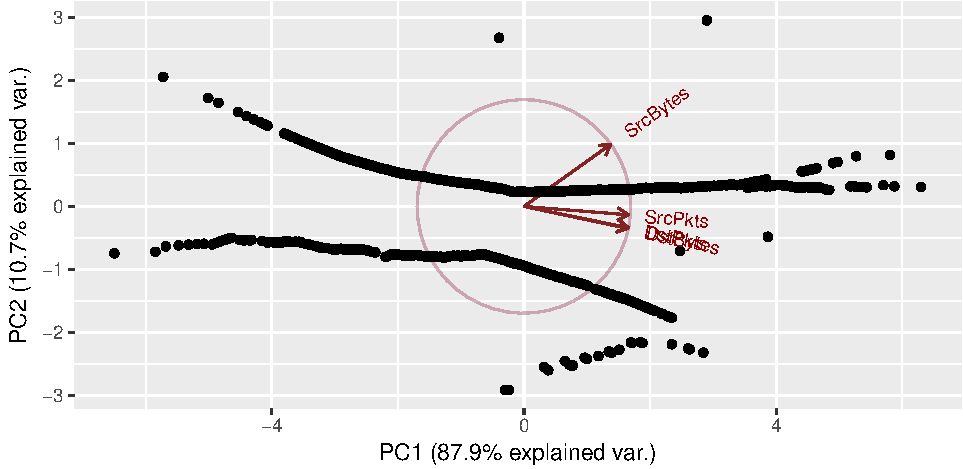
\includegraphics{thesis_files/figure-latex/unnamed-chunk-26-2.pdf}
\begin{verbatim}
Sport: 19239    Dport: 9153 
               PC1        PC2        PC3          PC4
SrcBytes 0.4400190  0.8125062 -0.3823817 -0.001104223
SrcPkts  0.5189497  0.1174251  0.8466938 -0.003489750
DstBytes 0.5179403 -0.4057384 -0.2640886 -0.705245607
DstPkts  0.5184712 -0.4017728 -0.2591352  0.708953621
Importance of components:
                          PC1    PC2     PC3     PC4
Standard deviation     1.8418 0.7037 0.33316 0.03695
Proportion of Variance 0.8481 0.1238 0.02775 0.00034
Cumulative Proportion  0.8481 0.9719 0.99966 1.00000
\end{verbatim}
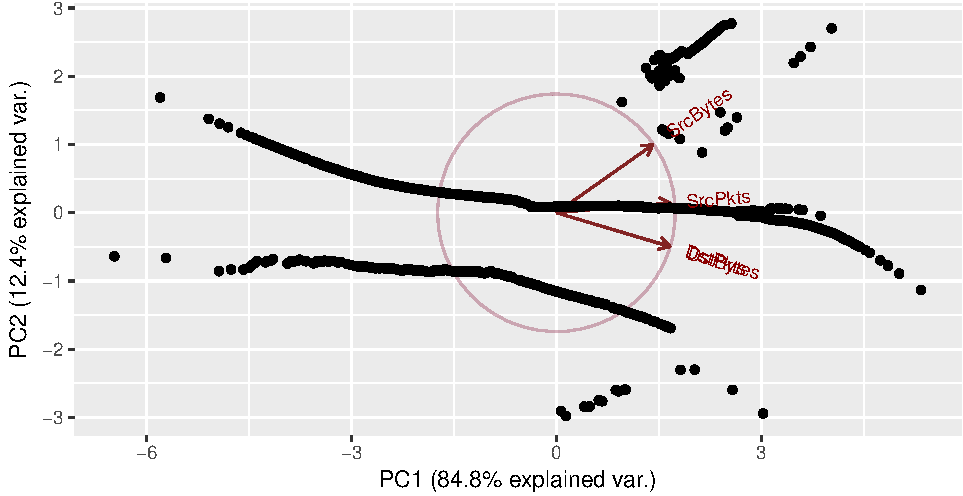
\includegraphics{thesis_files/figure-latex/unnamed-chunk-26-3.pdf}
\begin{verbatim}
Sport: 4243     Dport: 27 
               PC1        PC2        PC3          PC4
SrcBytes 0.3986539  0.8262979 -0.3978739  0.001762539
SrcPkts  0.5268775  0.1487193  0.8367993  0.007045781
DstBytes 0.5300998 -0.3876467 -0.2708012  0.703840168
DstPkts  0.5314785 -0.3805842 -0.2610173 -0.710321243
Importance of components:
                          PC1    PC2     PC3     PC4
Standard deviation     1.7727 0.8343 0.40033 0.03406
Proportion of Variance 0.7856 0.1740 0.04007 0.00029
Cumulative Proportion  0.7856 0.9596 0.99971 1.00000
\end{verbatim}
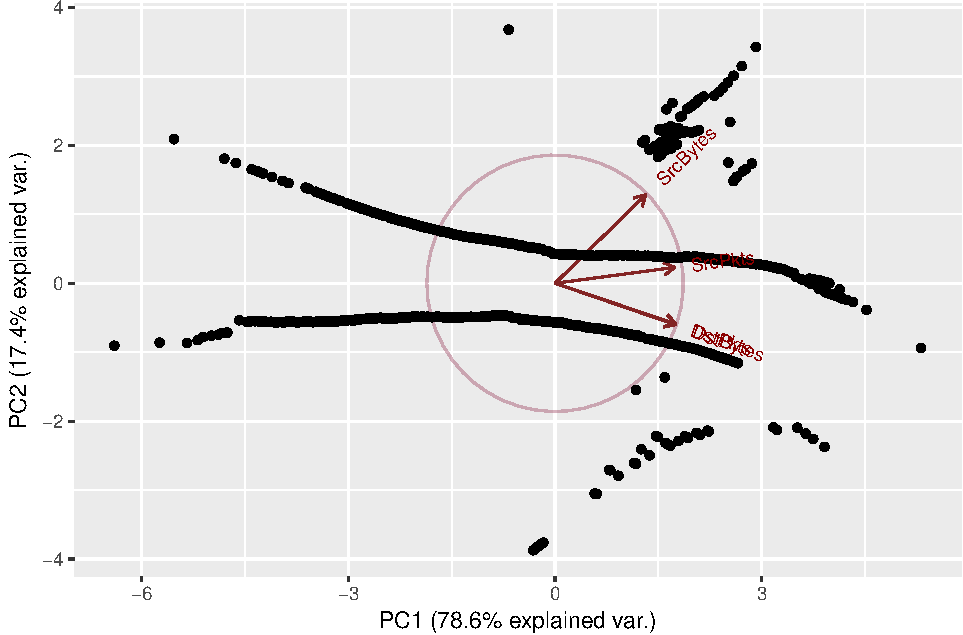
\includegraphics{thesis_files/figure-latex/unnamed-chunk-26-4.pdf}
\begin{verbatim}
Sport: 4243     Dport: 10290 
                PC1         PC2        PC3          PC4
SrcBytes -0.4146349  0.86007431 -0.2972268 -0.002501828
SrcPkts  -0.5225073  0.04229265  0.8514240 -0.016572825
DstBytes -0.5257892 -0.36545098 -0.3181251 -0.699133556
DstPkts  -0.5278350 -0.35345310 -0.2924547  0.714794623
Importance of components:
                          PC1    PC2     PC3     PC4
Standard deviation     1.8125 0.7560 0.37528 0.05022
Proportion of Variance 0.8213 0.1429 0.03521 0.00063
Cumulative Proportion  0.8213 0.9642 0.99937 1.00000
\end{verbatim}
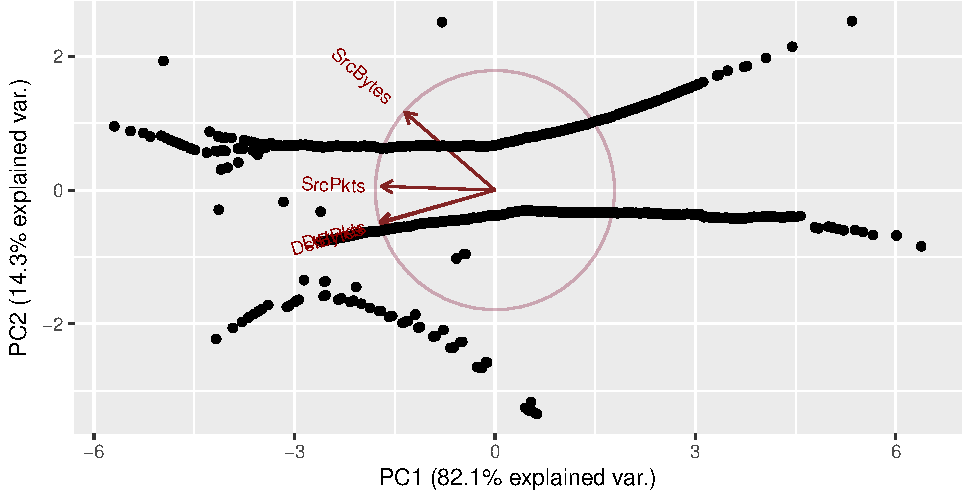
\includegraphics{thesis_files/figure-latex/unnamed-chunk-26-5.pdf}

\subsection{Interpretation}\label{interpretation}

In general the first two principal components explained most of the
variance (\textasciitilde{}90\%) for each of the port combinations. The
scatterplots of the principal components show clear horizontal patterns
in the 2nd principal component. This similar behavior, mirrored
throughout the top 10 most frequent ports, may be caused by the high
frequency of zeroes in the dataset. Recall, the first quartile of
observations for destination bytes and packets were all 0. This high
frequency of the same value (0) yields ties when performing the normal
scores transformation applied to the data, which may also cause the
horizontal behavior exhibited in every principal component analysis.

\backmatter

\chapter*{References}\label{references}
\addcontentsline{toc}{chapter}{References}

\markboth{References}{References}

\noindent

\setlength{\parindent}{-0.20in} \setlength{\leftskip}{0.20in}
\setlength{\parskip}{8pt}

\hypertarget{refs}{}
\hypertarget{ref-GLSmatrix2013}{}
Allen, G. I., Grosenick, L., \& Taylor, J. (2014). A generalized
least-square matrix decomposition. \emph{Journal of the American
Statistical Association}, \emph{109}(505), 145--159.

\hypertarget{ref-prior2014}{}
Alquier, V. C., Pierre; Cottet. (2014). Bayesian matrix completion:
Prior specification.

\hypertarget{ref-pca2012}{}
Bailey, S. (2012). Principal component analysis with noisy and/or
missing data.

\hypertarget{ref-EYM1987}{}
G.H. Golub, G. S., Alan Hoffman. (1987). A generalization of the
eckart-young-mirsky matrix approximation theorem. \emph{Linear Algebra
and Its Applications}, \emph{88-89}, 317--327.

\hypertarget{ref-fastALS2014}{}
Hastie, R. L., Trevor; Mazumder. (2014). Matrix completion and low-rank
svd via fast alternating least square.

\hypertarget{ref-hoff2009}{}
Hoff, P. D. (2009). \emph{A first course in bayesian statistical
methods}. Springer-Verlag New York.

\hypertarget{ref-smoothParafac2016}{}
Tatsuya Yokota, A. C., Qibin Zhao. (2016). Smooth parafac decomposition
for tensor completion. \emph{IEEE Transactions on Signal Processing
Issue 20}, \emph{64}(20), 5423--5436.

\hypertarget{ref-netflix2009}{}
Toscher, A., Jahrer, M., \& Bell, R. M. (2009). The bigchaos solution to
the netflix grand prize.

\hypertarget{ref-sparse2014}{}
Yang, D., Ma, Z., \& Buja, A. (2014). A sparse singular value
decomposition method for high-dimensional data. \emph{Journal of
Computational and Graphical Statistics}, \emph{23}(4), 923--942.
Retrieved from \url{https://doi.org/10.1080/10618600.2013.858632}

\hypertarget{ref-gibbs2010}{}
Zhou, M., Wang, C., Chen, M., Paisley, J., Dunson, D., \& Carin, L.
(2010). Nonparametric bayesian matrix completion. In \emph{2010 ieee
sensor array and multichannel signal processing workshop} (pp.
213--216).


% Index?

\end{document}
